% Based on Andrews Ex 7.3
\begin{question}
Implement a program to sort $n$ integers using a pipeline of $n$
components, as depicted below (note that the value of $n$ is known in
advance).
%
\begin{center}
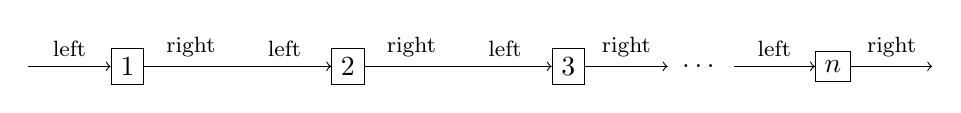
\begin{tikzpicture}[xscale = 2.8]
\draw(0,0) node[draw] (0) {1};
\draw[<-] (0) -- node[above]{\footnotesize\scalastyle left} ++(-0.45,0);
%
\draw(1,0)  node[draw] (1) {2};
\draw[->] (0) -- node[above,near start]{\footnotesize\scalastyle right}
  node[above,near end]{\footnotesize\scalastyle left} (1);
%
\draw(2,0)  node[draw] (2) {3};
\draw[->] (1) -- node[above,near start]{\footnotesize\scalastyle right}
  node[above,near end]{\footnotesize\scalastyle left} (2);
%
\draw[->] (2) -- node[above]{\footnotesize\scalastyle right} ++(0.45,0);
%
\draw(2.6,0) node {\ldots};
%
\draw(3.2,0) node[draw] (n) {$n$};
\draw[<-] (n) -- node[above]{\footnotesize\scalastyle left} ++(-0.45,0);
\draw[->] (n) -- node[above]{\footnotesize\scalastyle right} ++(0.45,0);
\end{tikzpicture}
\end{center}
%
Each component should receive a stream of values on its \SCALA{left} channel,
keep the largest, and pass the rest to the next component, via its
\SCALA{right} channel.  Each component should hold at most two values at any
time: the most recently received value and the largest seen so far.  The end
of the input stream should be signalled by the input channel being closed.  At
the end, the sorted values should be output on the right-most channel, and
that channel closed.

Implement a testing rig for the sorting network.

Would your network sort more than $n$ input values?

How many messages are sent in total (as a function of~$n$)?

Assuming each component runs on its own processor, how does the execution time
depend upon~$n$ (using $O(\_)$ notation).  In other words, how does the length
of the longest totally ordered chain of messages \( m_1 \prec m_2 \prec \ldots
\prec m_k \) depend on~$n$?  Optional: give an exact value for the length of
the longest such chain.
\end{question}

%%%%%

\begin{answerI}
My code is below.  I've chosen to have a function |apply| that returns the
network, and to make the |left| and |right| channels public; but there are
other ways of structuring the code.
%
\begin{scala}
/** A network to sort £n£ numbers, using a pipeline. */
class PipeSort(n: Int){
  /** A single node. */
  private def node(left: ?[Int], right: ![Int]) = thread("node"){
    var current = left?()
    repeat{
      val next = left?()
      if(current > next) right!next
      else { right!current; current = next }
    }
    right!current; right.endOfStream()
  }

  private val chans = Array.fill(n+1)(new SyncChan[Int])

  /** The input channel to the pipeline. */
  val left = chans(0)

  /** The output channel from the pipeline. */
  val right = chans(n)

  /** The sorting network. */
  def apply(): ThreadGroup =
    || (for(i <- 0 until n) yield node(chans(i), chans(i+1)))
}
\end{scala}

Testing can be done in the same way that we tested the Mergesort program in
the body of the chapter.

%% My testing code is below.  The |generator| injects the values from~|xs| into
%% the network; the |collector| deposits the outputs into~|ys|; at the end we
%% check that |ys| is a sorted version of~|xs|.  
%% %
%% \begin{scala}
%% import scala.util.Random

%% /** A testing rig for PipeSort. */
%% object PipeSortTest{
%%   /** Send values from £xs£ on £right£. */
%%   def generator(right: ![Int], xs: Array[Int]) = thread("generator"){
%%     for(i <- 0 until xs.length) right!xs(i)
%%     right.endOfStream()
%%   }

%%   /** Receive random numbers on £left£, and store in £ys£. */
%%   def collector(left: ?[Int], ys: Array[Int]) = thread("collector"){
%%     for(i <- 0 until ys.length) ys(i) = left?()
%%   }

%%   /** Perform a single test: pass in random numbers; record output; check
%%     * output is sorted version of input. */
%%   def doTest = {
%%     val N = 100; val xs = Array.fill(N)(Random.nextInt)
%%     val ys = new Array[Int](N)
%%     val ps = new PipeSort(N)
%%     // Run system
%%     run(generator(ps.left, xs) || ps() || collector(ps.right, ys))
%%     assert(xs.sorted.sameElements(ys))
%%   }

%%   def main(args : Array[String]) = {
%%     for(i <- 0 until 500){ doTest; if(i%10 == 0) print(".") }
%%     println()
%%   }
%% }
%% \end{scala}

The network would actually sort~$n+1$ values.\footnote{Thanks to Alfonso Bueno
  Orovio for this observation.}  After $n$ inputs, we can get to a state where
every node is holding a value; but no value will be output until either the
input channel is closed, or another value is input; if another value is then
input, it will be treated correctly.

However, the network can't handle more than $n+1$ inputs in general.  Consider
$n+2$ inputs where the final input is the smallest.  The first output will be
the smallest of the first $n+1$ inputs, which is incorrect.

There are $n(n+1)$ messages in total (for $n$ inputs): each of the $n$ values
is passed on each of the $n+1$ channels.

There are $O(n)$ sequentially ordered messages.  The point is that node~$k$
can receive a message concurrently with node~$k+1$ sending a message.  This
means that if node $k$ now holds two values, it can immediately send one to
node~$k+1$.  Thus it  takes about $2n$ rounds for all values to be input.  It
then takes another $O(n)$ rounds (actually about $3n$) for the final value to
propagate along the pipeline.

More precisely, there are $5n-3$ sequentially ordered messages (assuming $n >
2$):
\begin{itemize}
\item the first node receives $n$ messages and sends $n-1$ messages before
  detecting the input channel is closed; 

\item at this point, the second node holds two values (if $n>2$): it passes
  one on, receives the final value from the first node, passes one value on,
  then detects that its input channel is closed;

\item similarly, there are three communications between each node~$n_k$ 
  detecting its input channel is closed, and the next node $n_{k+1}$ detecting
  its input channel is closed;

\item the final node does a final output. 
\end{itemize}
% 
This gives a total of $(2n-1) + (n-1)\times 3 + 1 = 5n-3$ (for $n>2$).  
\end{answerI}
